%	Copyright (C) 2013 Systems Engineering Group
%
%	CHANGELOG:
%       2005-10-10 - corrected and extended. 
%       2013-01-28 - adjusted sections and explanation
%


\documentclass[a4paper,10pt,twoside]{article}
\usepackage{blindtext}
\pagestyle{headings}
\usepackage{a4wide}
\usepackage{graphicx}
\usepackage[font=small,labelfont=bf]{caption}
\usepackage{caption}
\usepackage{subcaption}
\usepackage[colorlinks,hyperfigures,backref,bookmarks,draft=false]{hyperref}
\usepackage[utf8]{inputenc}

\usepackage{listings}
\usepackage{color}

\definecolor{codegreen}{rgb}{0,0.6,0}
\definecolor{codegray}{rgb}{0.5,0.5,0.5}
\definecolor{codepurple}{rgb}{0.58,0,0.82}
\definecolor{backcolour}{rgb}{0.95,0.95,0.92}

\lstdefinestyle{mystyle}{
	backgroundcolor=\color{backcolour},   
	commentstyle=\color{codegreen},
	keywordstyle=\color{magenta},
	numberstyle=\tiny\color{codegray},
	stringstyle=\color{codepurple},
	basicstyle=\footnotesize,
	breakatwhitespace=false,         
	breaklines=true,                 
	captionpos=b,                    
	keepspaces=true,                 
	numbers=left,                    
	numbersep=5pt,                  
	showspaces=false,                
	showstringspaces=false,
	showtabs=false,                  
	tabsize=2
}

\lstset{style=mystyle}
\title{Levenshtein Distance}
%\author{John Doe\\Magic Department, Richard Miles University}
\author{Ansh Rupani \\ \\ \\Matrikel. Nr: 4676365 \\ \\ \\Study Program: Master of Science in Distributed Systems Engineering \\ \\ \\Email: ansh.rupani@tu-dresden.de}
%\date{\today}

\begin{document}

\maketitle


%\begin{abstract}
%There has been an ever growing demand of multi-core architectures for achieving higher levels of concurrency. Multi-threaded programing faces new challenges on throughput-oriented architectures like GPUs. The immense performance pressure on synchronization primitives like mutexes on tasks like memory allocation is unimaginable due to the extremely high number of threads in such architectures. The authors in \cite{gelado2019throughput} propose various concurrent programming techniques for GPU architectures to support better dynamic memory allocation.
%
%The authors have build their memory allocator with the support of other improvements they have proposed in the paper. They have proposed bulk semaphores, a generalized variant of counting semaphores which supports the case when multiple threads operate on a semaphore concurrently. A better approach for synchronization mechanisms like Read-Copy-Update has been proposed where multiple threads are allowed to access the critical section of the program simultaneously. Also, techniques to delegate deferred reclamation to threads which are already blocked have been proposed. All these proposed techniques when combined together contribute towards a highly throughput-oriented GPU memory allocator, which performs 16.56 times better than the CUDA based memory allocator in terms of allocation rates.
%\end{abstract}

\pagebreak

\tableofcontents

\newpage

\section{Problem Description}

Levenshtein distance, also known as the edit distance is an algorithm  used to measure the difference between two strings. In short, it can be taken as the number of minimum edits required to convert string 1 into string 2. Normally, the allowed edits are:\\ \\
1) Insert a character\\
2) Remove a character\\
3) Replace a character\\ \\
For example, if string 1 is ``chicken" and string 2 is ``kitchen", the edit distance is 4, because to make both the strings equal, `c' in ``chicken" can be changed to `k', `h' in ``chicken" can be removed, `t' and `h' in ``kitchen" can be removed. Thus, because of these 4 changes, the edit distance is 4. It is assumed that the cost for implementation of any of the edits is the same. It finds applications in fields such as plagiarism detectors.

\section{In Depth Analysis of the Unoptimized Algorithm}

In the provided algorithm, the idea is to process all characters one by one starting from one particular end of the strings (here, the right end). If the last characters of the strings are the same, these characters are ignored and a fresh recursive call is made without these characters and minimized string length(decremented by 1). Else, it checks whether the beginning of the string is same as the end of the string. In this case, function call is made to \textit{dist} which returns the number of elements between the first and last element of the other string. If the last characters are not the same, a recursive call is made to obtain the minimum cost out of all three possible operations of insert, remove and replace. To signify the insert operation, it is similar to recurring for \textit{str1.length()} and \textit{str2.length() - 1}. For the remove operation, it is same as recurring for \textit{str1.length() - 1} and \textit{str2.length()}. Similarly, for the replace operation, we recur for \textit{str1.length() - 1} and \textit{str2.length() - 1}. 

\section{Complexity Analysis}
The complexity of this algorithm is exponential. This algorithm requires multiple subproblems to be solved, repeatedly. $O(3^{len})$ operations might be required in the worst case. Such a worst case arises when there is no match between any of the characters of any string.
\begin{figure}
	\centering
	\begin{subfigure}[t]{0.3\columnwidth}
		\centering
		\scalebox{0.95}{\includegraphics[width= \linewidth]{paper/pic1.png}}
		\label{fig:bulk}
		\caption{}
		\label{fig:bulk}
	\end{subfigure}
	\begin{subfigure}[t]{0.3\columnwidth}
		\centering
		\scalebox{0.94}{\includegraphics[width= \linewidth]{paper/pic2.png}}
		\vspace{0.1 em}
		\label{fig:rcu}
		\caption{}
		\label{fig:rcu}
	\end{subfigure}	
	\caption{(a) Normal DP Strategy (b) Diagonal DP Strategy \cite{yang2014parallel}}
	\vspace{-1.5em}
\end{figure}
\section{Optimization}
On observing the recursive call graph of the problem, one could notice that there are various similar subproblems which are solved in the algorithm. The overlapping subproblems are worked upon again and again, thereby increasing the runtime of the algorithm. Therefore, to avoid such recomputations, dynamic programming approach seemed to make a lot of sense. This is made possible by storing the solutions of the subproblems in a two dimensional array. Therefore, whenever the same subproblem is called, the respective solution can be fetched from this matrix. Further, an iterative version of the algorithm would be more efficient in terms of the execution time. Figure 1a shows the DP matrix, where the last element DP[str1.length()][str2.length()] gives the final edit distance. The code snippet which helps in filling this matrix is given in Listing 1. In this matrix, the first column and row are filled first, which also help in initializing the process for the next calculations as there is a clear dependency amongst the elements. More on this dependency is discussed in Section 5.1.

\section{Parallelization Strategies}
To parallelize the optimized algorithm, various approaches were tried. The first one was to introduce data independency in the algorithm and exploit the fact that while diagonally iterating over the DP matrix, the individual elements in the diagonal can be calculated individually. Then, an approach is discussed wherein an optimized recursive task is assigned for each of the diagonal elements. Then, an approach is presented especially targeting large inputs.

\subsection{Introduction of Data Independency and Diagonal Matrix Iteration (a.k.a. Most Optimized Strategy)}
The optimized algorithm was iterative. The DP matrix was iterated over element by element in a manner such that after iterating through all the elements of the first row from left to right, the second row was approached in a similar manner and so on. In this version, to introduce parallelism, it was necessary that the present element that is being worked out does not depend on a previous element in a way that would hamper the benefits. This was not the case because the calculation of the $(i, j)^{th}$ was dependent upon the $(i, j-1)^{th}$ element, $(i-1, j)^{th}$ element and $(i-1, j-1)^{th}$ element. This also means that we can only proceed to calculate the $(i, j)^{th}$ element once the other three elements are calculated. Listing 1 shows the code snippet for the DP problem.\\
\begin{lstlisting}[language=c++, caption=Code Snippet For DP Version]
if (i==0) 
dp[i][j] = j;

else if (j==0) 
dp[i][j] = i; 

else if (str1[i-1] == str2[j-1]) 
dp[i][j] = dp[i-1][j-1]; 

else
dp[i][j] = 1 + min(dp[i][j-1], dp[i-1][j], dp[i-1][j-1]);
\end{lstlisting}
To bring data independency into effect for obtaining parallelism, a decision was made to \textbf{\textit{diagonally iterate}} the DP matrix. This decision is better understood with the help of an example, as shown in Figure 1b. On can notice that elements in an individual diagonal can be independently at the same time because there is no dependency amongst them when that particular diagonal is being iterated upon. In the figure, elements in a particular diagonal (having the same colour) can be calculated independently when iterating over these individual elements. Such iteration would empower \textit{data parallelism}\\ \\
This gives a motivation for parallelism. In a diagonal, the calculation for individual elements can be assigned to individual threads.

For doing this, an outer loop was created to iterate over the total diagonals in the matrix. Based on the value of the \textit{count} variable, which stores the number of elements in that particular diagonals, and the number of threads available (capped by the number of cores available), a decision is made whether to assign individual element calculation to a thread or assign the calculation of a set of elements to a thread. Also, the number of threads which should be involved for a particular diagonal is also capped by the minimum of number of elements in that diagonal and the number of cores available. In the \textit{doWork} method (assigned to threads), the work shown in Listing 1 is done for each element individually. We don't go on further until all the threads have completed their job, because it is necessary to have the elements of the current diagonal in hand before moving on to the next diagonal. Also, the DP matrix is a globally shared matrix. But there is no need to protect it with locks, thanks to the data independency introduced by iterating diagonally. Therefore, this approach is a \textit{lock-free} approach.

However, this approach did not give expected results and one of the reasons could be that the overhead of creating and introducing some synchronization for the threads was more than the actual task of filling the DP matrix elements. Also, the scalability is capped by the number of elements in the diagonals, thereby overpowering the number of cores available. Also, even the use of threadpool didn't help much, due to similar reasons.

\subsection{Assigning Atleast a Fixed Number of Elements to the Threads (a.k.a. Large Strategy)}
After observing the results, there was no speedup obtained with increase in the number of cores (also the number of threads). Therefore, the amount of work to be given to particular threads (especially supposed to be helpful for large inputs) was decided at runtime, based on the number of elements to be calculated in a particular diagonal and the number of threads available. Only if a particular diagonal had more than a threshold number of elements to be calculated, multi-threading was used and the tasks assigned were assigned at runtime. In any other case, only a single thread was created to work on all the elements of a particular diagonal. This should have given better results for scalability, but the algorithm was again so fast that the overhead of introducing multi-threading was more. The minimum factor was also modifiable, but even after playing with it, better results could not be observed in terms of scaling.

\subsection{Assigning Recursive Tasks to Threads (a.k.a. Scaled Strategy)}
To increase the workload on individual threads, while still iterating diagonally, the calculation of the individual elements of a particular diagonal is done recursively, individually, but, with minimum optimization. This means that instead of calculating the cost three possible edits recursively, only two such calls are made recursively, for each individual diagonal element. The cost for the third edit possibility is picked up from the DP matrix (therefore, limiting optimization). Thereafter, the minimum cost is calculated after obtaining all three values. This version is still very optimized and better as compared to the originally provided, however, we compromise on optimization to gain scalability in this case. But on observing speedup in this case, the conclusion which we came at earlier, that there is no speed up in the initial approach due to less work being assigned to the threads, seems to be true. 

\subsection{Using Threads For Each Individual Recursive Call in The Normal Recursive Code}
Another approach which was considered was to parallelize individual recursive calls in the normal recursive code, exploiting the fact that there was no shared data structure among the parallelized tasks. But the factor which made it difficult was that the other thread which would have been based normally on the outputs of the minimum of the previous three recursive calls. This version was not evaluated on the system because of some issues arising out of the handling of this factor. However, this version is also available on github.


\begin{figure}[t]
	\centering
	\scalebox{0.9}{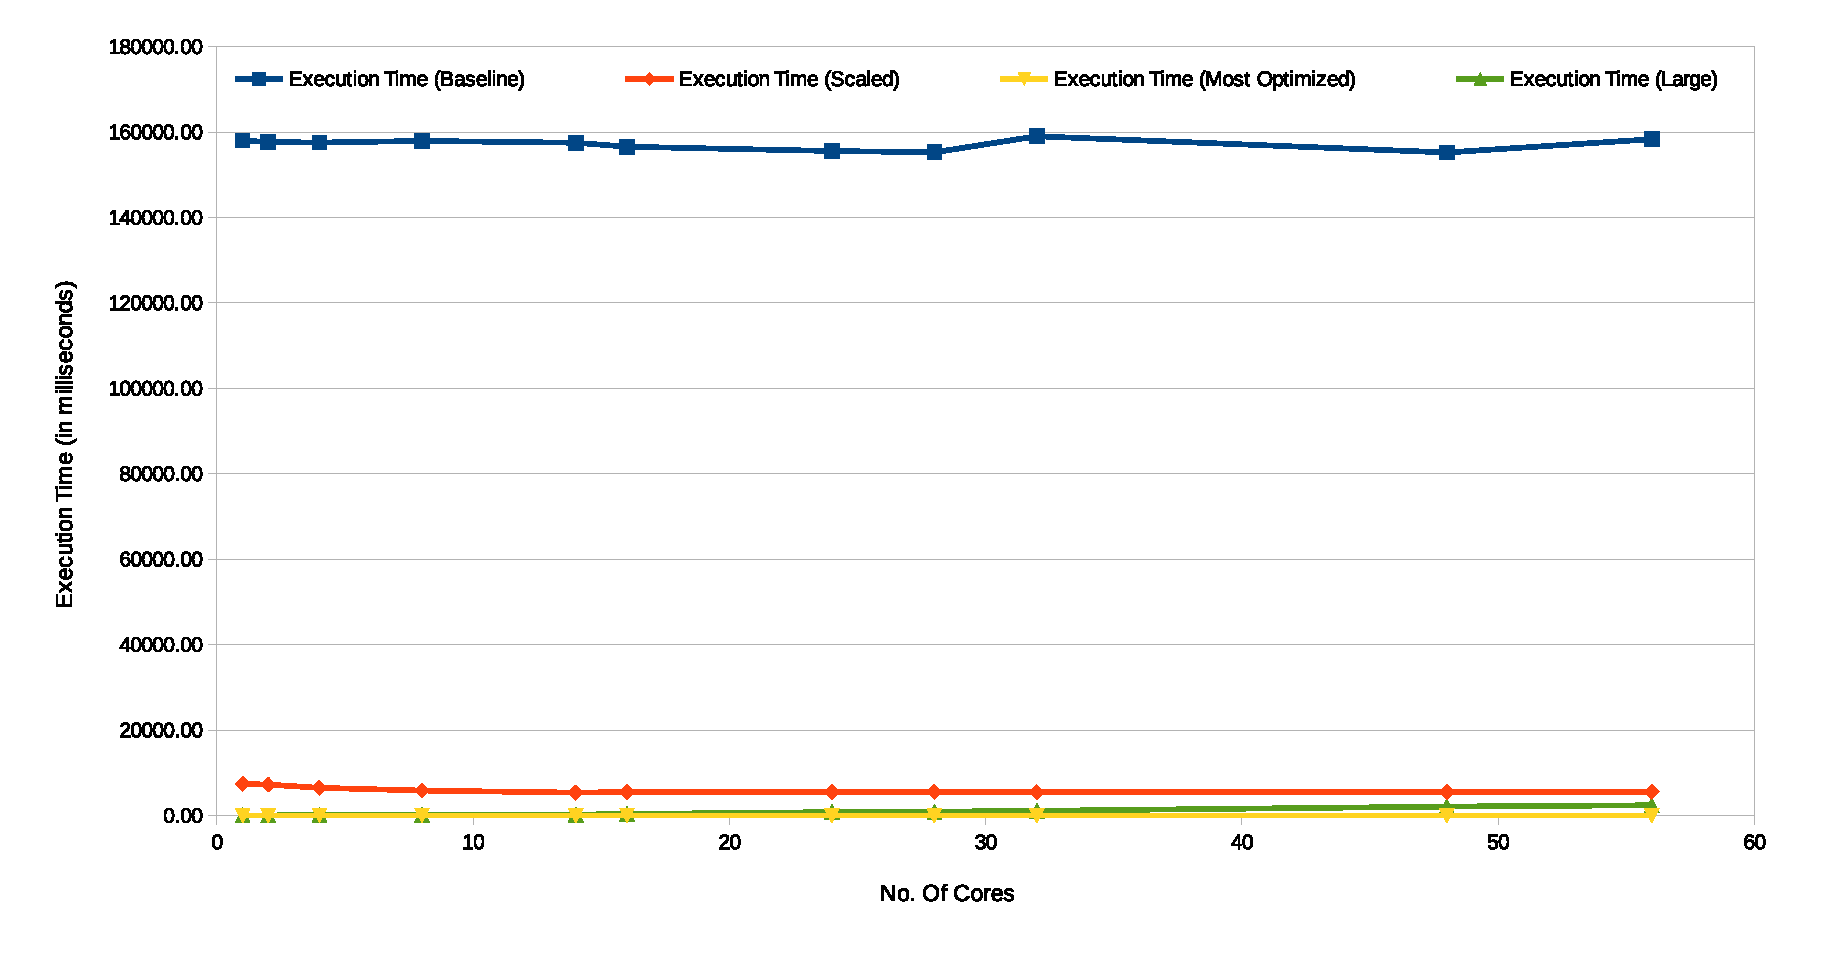
\includegraphics[width= \linewidth]{paper/exec.eps}}
	\caption{Execution Time (in ms) for Various Strategies}
	\label{fig:ualloc}
\end{figure}

\section{Comparison and Evaluation}

Figure 2 and 4 show the execution time (with respect to baseline) and speed up (with respect to single threaded performance) of various strategies, while Figure 3 shows the speed of the \textit{scaled} strategy with respect to baseline. Baseline is the provided C++ algorithm. The most promising strategy for the demonstration of scaling was the one discussed in Section 5.3. Assigning decently heavy tasks to the threads while still keeping the algorithm optimized as compared to the baseline helped to obtain such speedup. However, the execution time becomes constant after a certain number of cores. This happens because of the reason discussed in Section 5.3 itself. The number of threads are capped by the number of elements in a particular diagonal, irrespective of the number of cores available. Therefore, bigger inputs make more sense for such tasks. But due to the very large size of the other test inputs (mopp-2018-t2-levenshtein-large) and because of reduced optimization, the evaluation system would timeout in this case. Therefore, the algorithm would not scale up after a certain number of cores. The average effect of scaling across the diagonals (with less and more number of elements each) saturates at a certain point.

The other approach discussed in Section 5.2 scaled upto a total of two cores, and not further. In this case, the threshold limit as discussed above depends on the number of cores. To accommodate more parallelism with more available cores, this threshold is set to decrease for every increase in the number of cores. But still, the speedup is inverted because waiting for the threads is more expensive than actually calculating the cost for the individual set of elements in the threads. Even after controlled disposition of tasks based on the threshold, no gradual scale up is observed. The formula for the threshold was changed to being constant as well as increasing with the number of cores, still, no specific speedup was observed. 

For the most optimized case, as discussed in Section 5.1, due to the reasons already stated above, no scaling could be obtained. the execution time mostly remained constant. 

Further, the DP based approach was already so much optimized that there was very less scope of introducing parallelism.

\begin{figure}[t]
	\centering
	\scalebox{0.9}{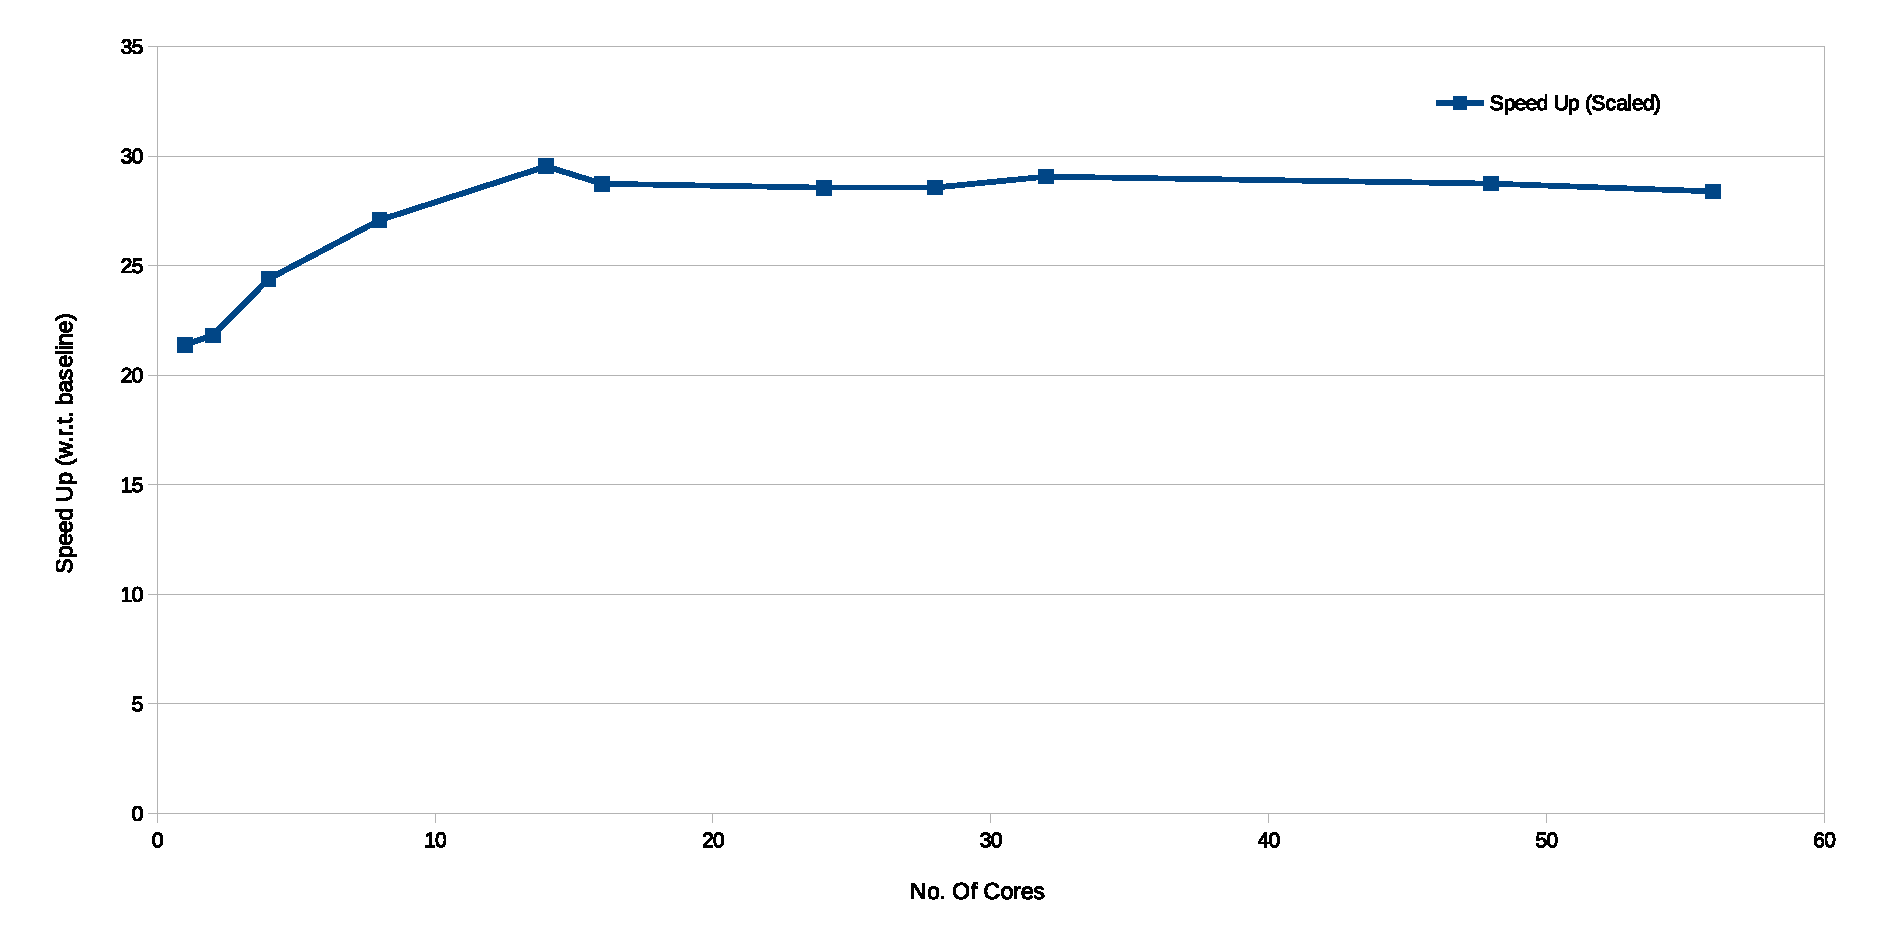
\includegraphics[width= \linewidth]{paper/speed2.eps}}
	\caption{Speed Up For The Scaled Strategy (Ref. Section 5.3)}
	\label{fig:ualloc}
\end{figure}

\begin{figure}[t]
	\centering
	\scalebox{0.9}{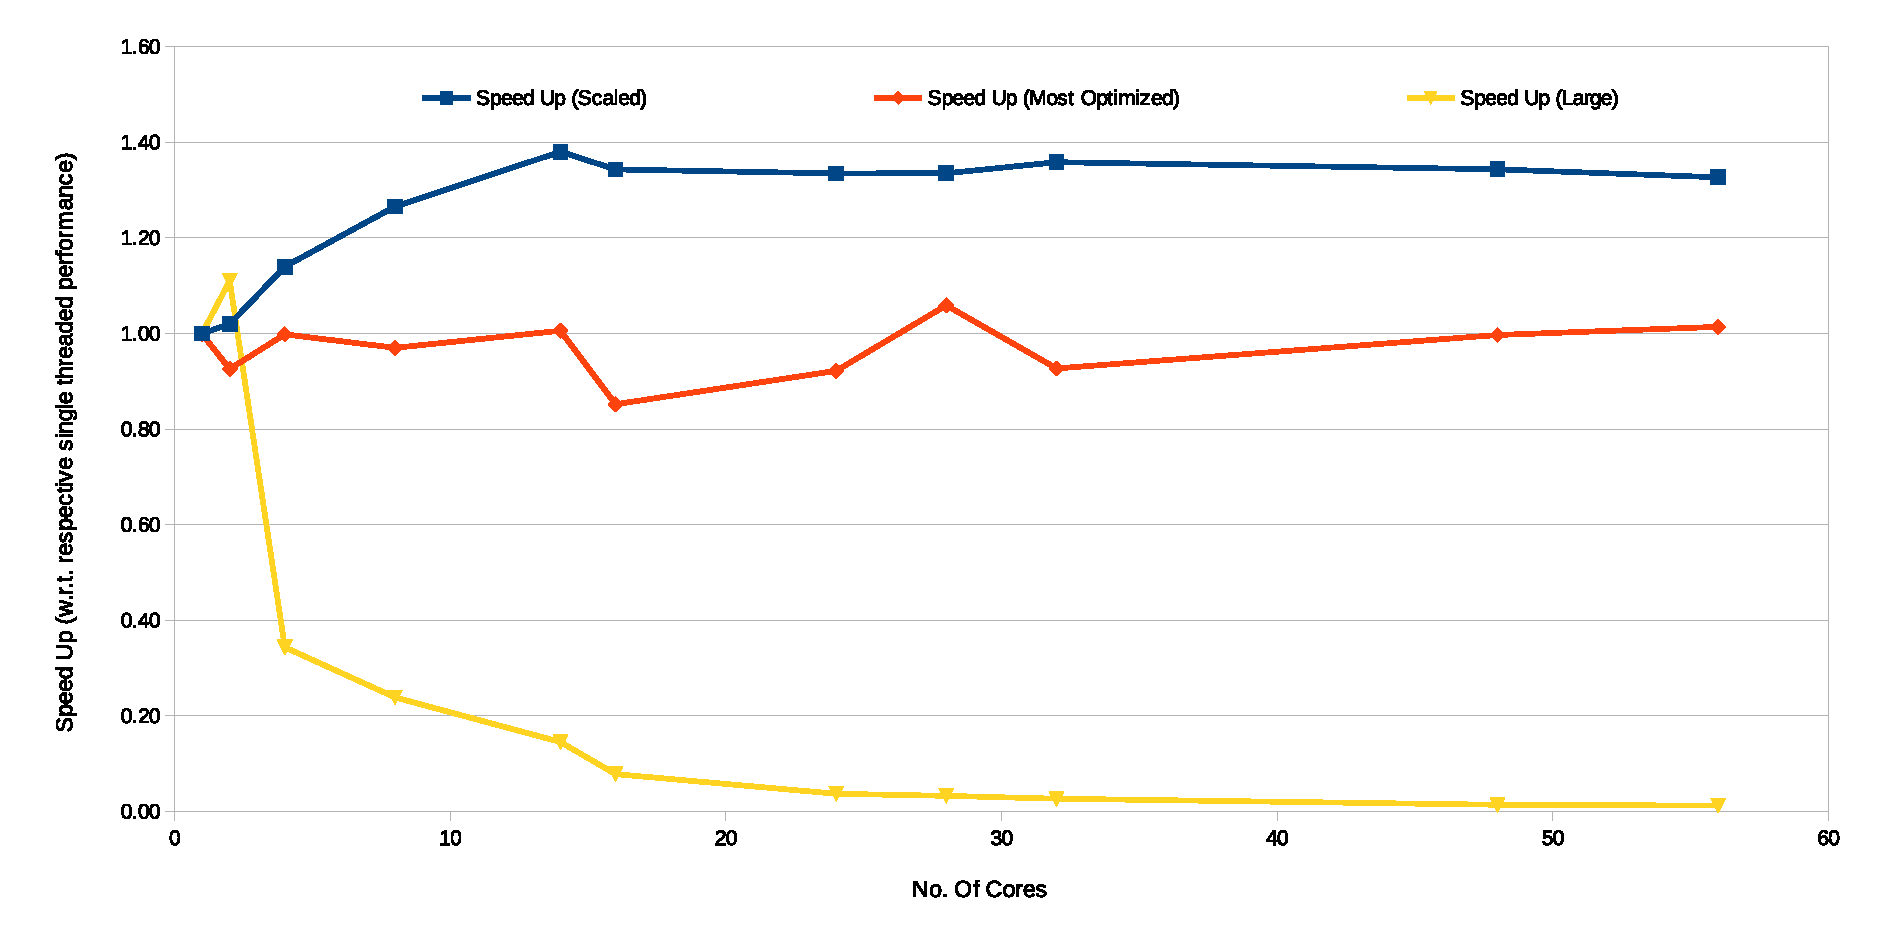
\includegraphics[width= \linewidth]{paper/speed1.eps}}
	\caption{Speed Up For Various Strategies w.r.t. Respective Single Threaded Performance}
	\label{fig:ualloc}
\end{figure}


\section{Speed Up Discussion and Analysis of Amdahl's Law}
Amdahl's law states the maximum possible theoretical speed up for a task that can be attained by using all available cores. It suggests that the sequential part of the task limits the speed up. In Eq. (1), \textit{A} is the attainable speedup, \textit{p} is the fraction of the task that can be parallelized and \textit{n} is the number of cores. 
\begin{equation}
	A = \frac{1}{(1-p) + p/n}
\end{equation}

Considering the baseline vs the \textit{Scaled} version, the speed up is as follows: 

\begin{equation}
Speed~Up~_{28~cores} = \frac{158032187}{5531196.67} = 28.6
\end{equation}

\begin{equation}
Speed~Up~_{56~cores} = \frac{158032187}{5565839.33} = 28.4
\end{equation}


The speed up is nearly constant because of the reasons discussed above.
If we see the performance of most optimized version, the speed up is enormous, majorly due to the optimizations and DP. The difference in values is because of random thread overheads and due to reasons already explained above.
\begin{equation}
Speed~Up~_{28~cores} = \frac{158032187}{2866} = 60195
\end{equation}

\begin{equation}
Speed~Up~_{56~cores} = \frac{158032187}{2412} = 57634
\end{equation}

However, using Eq. (1), following are the values for the parallel factor:

\begin{equation}
p~_{28~cores~(w.r.t.~baseline)} =  1
\end{equation}

\begin{equation}
p~_{56~cores~(w.r.t.~baseline)} =  0.98
\end{equation}

\begin{equation}
p~_{28~cores~(w.r.t.~single~threaded~in~scaled~version)} =  0.26
\end{equation}

\begin{equation}
p~_{56~cores~(w.r.t.~single~threaded~in~scaled~version)} =  0.25
\end{equation}


Though the \textit{p} factor w.r.t. the baseline should not be evaluated, it is still presented. By observing the \textit{p} values for 28 and 56 cores in Eq. (8) and (9), it can be seen that the values are similar, which normally is the case due to the cap in scalability infused by the sequential part of the task. The lesser speed up and thereby smaller \textit{p} value in 56 cores attributes to the fact discussed above, according to which the speed up is limited by the average number of elements in the diagonals.

\section{Appendix}

\begin{table}[h]
	\centering
	\scalebox{0.5}{\begin{tabular}{|l|l|l|}
			\hline
			\multicolumn{1}{|c|}{\textbf{Measurement}} & \multicolumn{1}{c|}{\textbf{Git Hash}} & \multicolumn{1}{c|}{\textbf{Evaluation URL}}                                                                                         \\ \hline
			Baseline                                   & cc67243                                & https://cds-lab-2019.netlify.com/logs/ef708123629f4ecf11cddda8fda3989645f7f572839455d588628a01a414a10b/2019-06-18T22:07:19+02:00.log \\ \hline
			Most Optimized (Sec. 5.1)                  & abb86fe                                & https://cds-lab-2019.netlify.com/logs/ef708123629f4ecf11cddda8fda3989645f7f572839455d588628a01a414a10b/2019-06-20T13:51:18+02:00.log \\ \hline
			Scaled (Sec. 5.2)                          & 558a65e                                & https://cds-lab-2019.netlify.com/logs/ef708123629f4ecf11cddda8fda3989645f7f572839455d588628a01a414a10b/2019-06-20T23:09:00+02:00.log \\ \hline
			Large (Sec. 5.3)                           & 558a65e                                & https://cds-lab-2019.netlify.com/logs/ef708123629f4ecf11cddda8fda3989645f7f572839455d588628a01a414a10b/2019-06-20T23:09:00+02:00.log \\ \hline
		\end{tabular}}
\end{table}

\bibliographystyle{alpha}
\bibliography{handin} 

\end{document}
